\documentclass[11pt]{article}
\usepackage{setspace}
\usepackage{gensymb}
\usepackage{minted}
\usemintedstyle{vs}
\usepackage[utf8]{inputenc}
\usepackage{graphicx}
\usepackage{mathtools}
\usepackage{amsmath}
\usepackage{multicol}
\usepackage{caption}
\usepackage{vmargin}
\usepackage{float}
\usepackage{circuitikz}
\usepackage{tikz}
\usetikzlibrary{shapes,arrows}
\usepackage{verbatim}

\usepackage{graphicx}
\graphicspath{ {./images/} }

\title{6.111 Project Proposal - Network-Attached Laser Projector}
\author{
  Jay Lang\\
  \texttt{jaytlang@mit.edu}
  \and
  Fischer Moseley\\
  \texttt{fischerm@mit.edu}
}
\date{26 October 2020}

\singlespacing
\begin{document}
\maketitle

\section{Abstract}
We propose a Network-Attached Laser Projector, which utilizes
a parallel-stack networking offload engine to connect to the
open internet and stream full-color vectorized images to an RGB
laser projector. The system will be capable of rendering
frames delivered to the projector through the networking stack,
which can be interfaced with directly as it is implemented in
raw hardware. With a direct connection to the TCP stack through the FPGA, we seek to demonstrate that high-bandwidth communication using existing standards can be accomplished with equivalent or better performance and efficiency relative to a traditional application processor implementation, and that lasers are really cool.

\section{Block Diagram}
\begin{figure}[H]
\centering
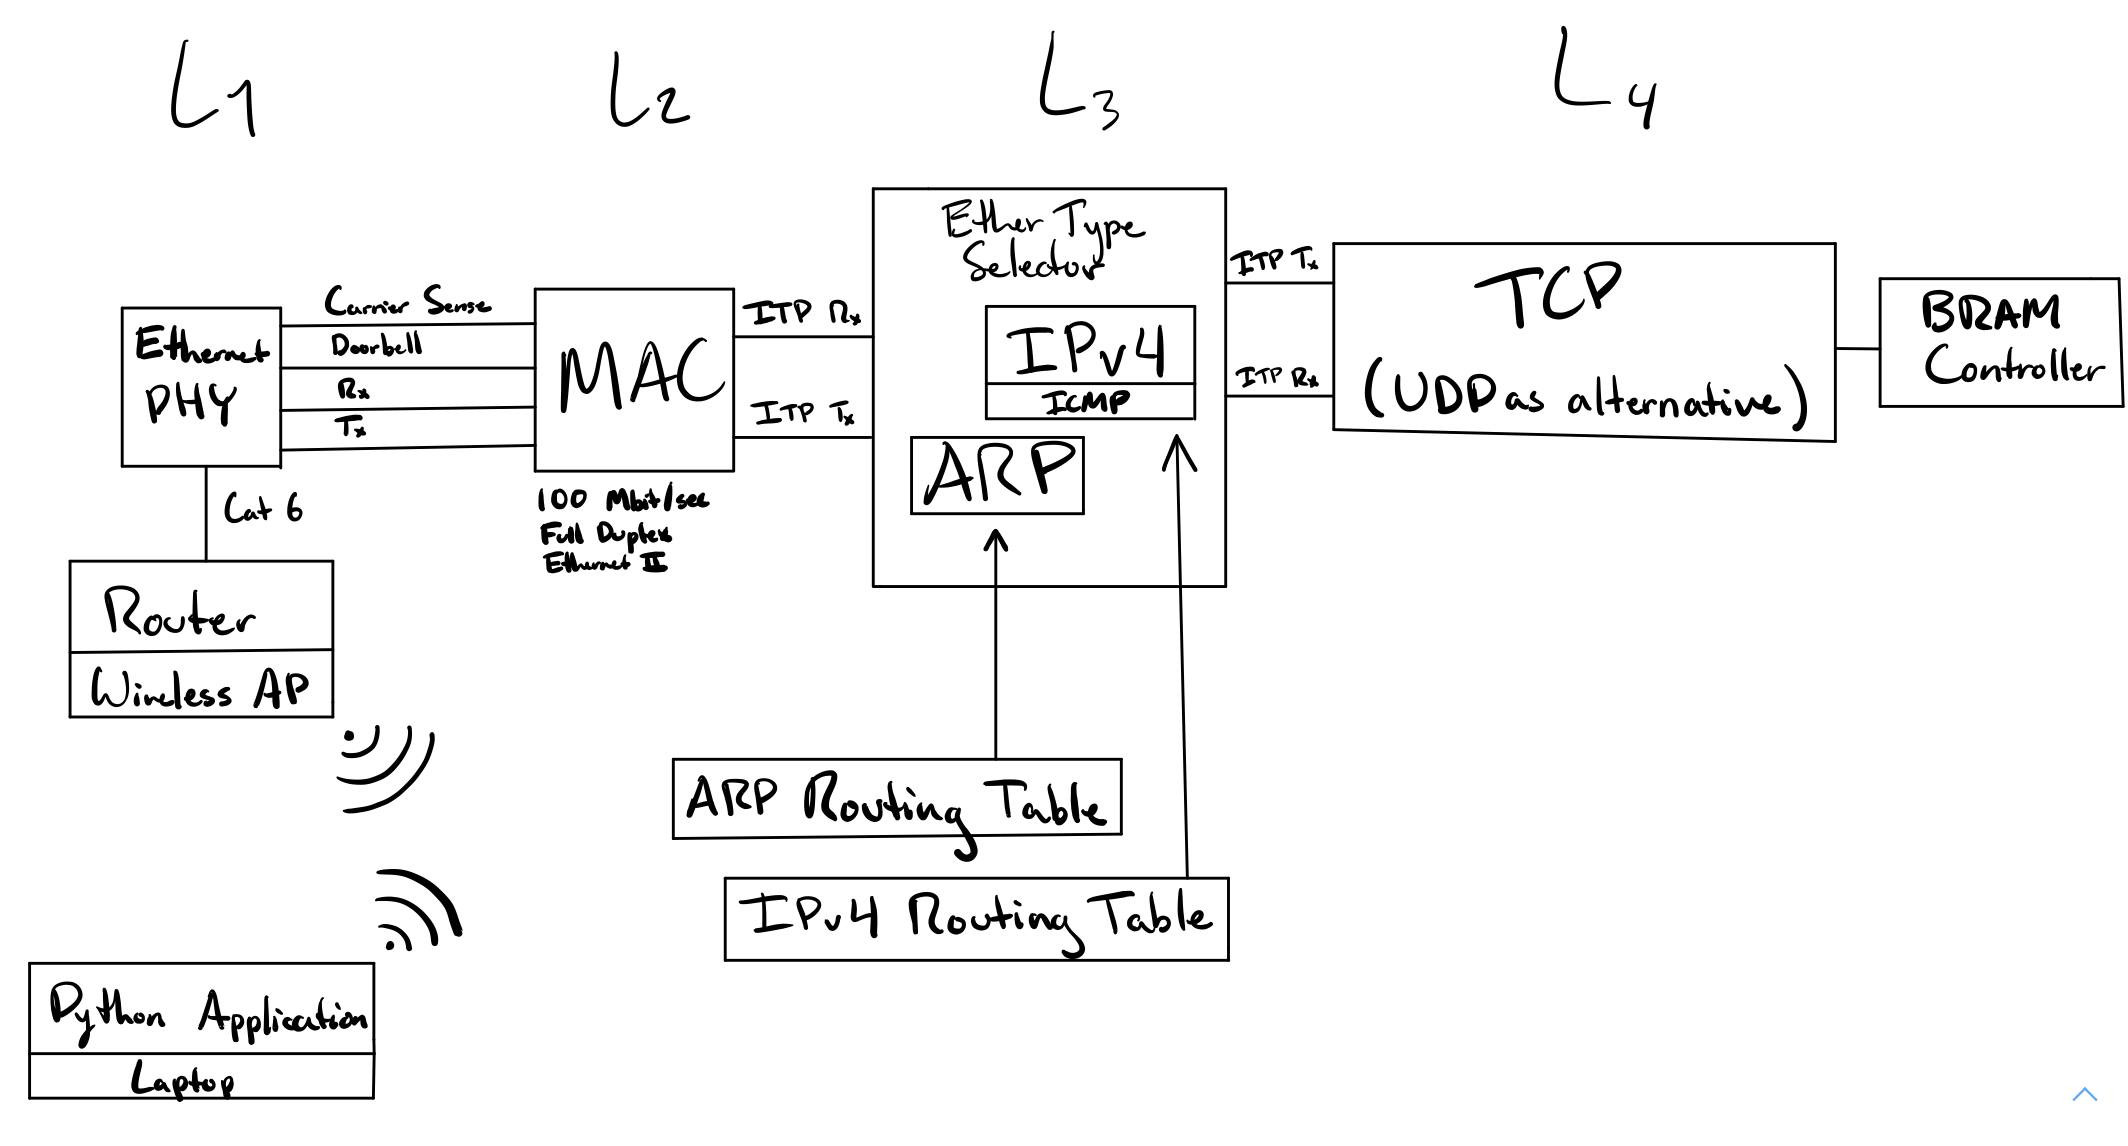
\includegraphics[width=1\textwidth]{network.jpg}
\caption{The networking stack, with wireless input from a laptop and output to the BRAM controller module.}
\end{figure}

\begin{figure}[H]
\centering
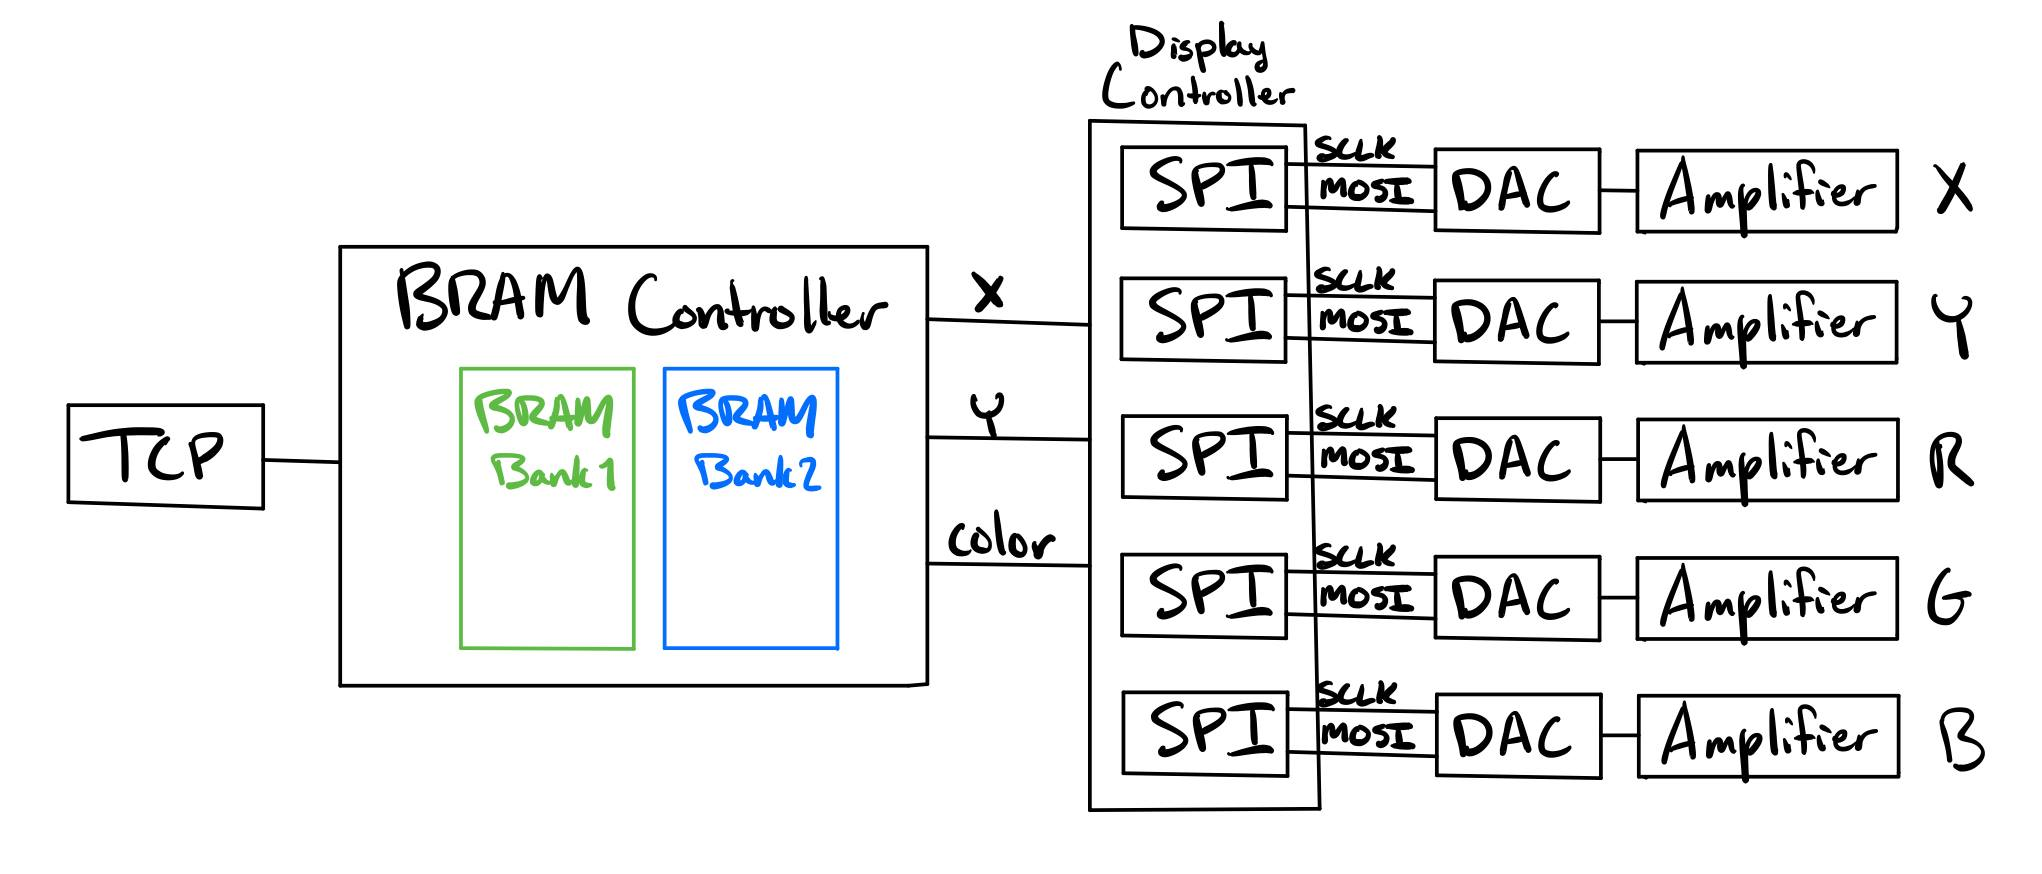
\includegraphics[width=1\textwidth]{laser.jpg}
\caption{The display logic and external components required, with input from the BRAM controller, and output to a set of SPI DACs.}
\end{figure}



\section{Networking Offload Engine (Jay)}

Jay will be implementing a Networking Offload Engine, whose role is to facilitate connecting to the open internet to stream laser data over the air. So far, we have implemented OSDI layer 2, and intend to continue to L3 at a minimum, with the target of reaching L4 via a subset of TCP.

\subsection{ITP}
As network layers are typically implemented in software, and often require buffering to support complex [de]encapsulation schemes, we expect to face design difficulties in adapting a more streaming oriented, hardware-capable model to widely used internet standards. To resolve this, we propose an Intermodule Transport Protocol (ITP), an AXI-like protocol with additional facilities to pause reception or transmission of packets mid-transmission to allow for potential pre-processing or signal generation to occur unimpeded.\newline

\noindent ITP demands the implementation of a receive hierarchy and a transmission hierarchy to unpack and deliver packets from/to the PHY. On the receiving side, $n$-bit ITP implements the following interface:
\begin{itemize}
    \item \texttt{data}: $n$ bits of data to receive
    \item \texttt{valid}: whether receiving data is valid
    \item \texttt{pause}: whether to stop receiving data, as data is still being streamed but a preprocessing operation is taking place
\end{itemize}

On the transmission end, ITP utilizes the following interface:
\begin{itemize}
    \item \texttt{data}: $n$ bits of data to transmit
    \item \texttt{valid}: whether this data is valid
    \item \texttt{pause}: whether the sender should stop updating valid, as the implementer is preprocessing data
\end{itemize}

\noindent Use of this system allows for a simple, common interface between components that maintains a streaming-oriented design and the hierarchical nature of modern networking stacks. As such, ITP appears in our block diagram and between all OSDI layers described below.

\subsection{Layer 1}
The FPGA comes with an Ethernet PHY rated for 100 Mbps. We will run this PHY at 100 Mbps with a reference clock of 50 MHz, utilizing full duplex operation. This PHY exports a carrier sense signal, as well as a TX-enable doorbell and a 2-bit wide RX and TX buffer.

\subsection{Layer 2}
We will implement a MAC per the IEEE 802.3 Ethernet II standard, running at the requisite 100 Mbps full duplex mode of operation. Separate modules are devised for RX and TX, each translating raw MAC packets to Ethernet frames. CRC32-BZIP2 is implemented as a separate module to complete the FCS, and such details are abstracted away from higher layers. \newline

\noindent This module is small, and can be tested using a combination of in-vivo debugging (e.g. via ILA) and software sniffing tools such as Wireshark over a direct Ethernet connection. We have already implemented this layer and successfully tested it via these means, including during full-duplex operation.

\subsection{Layer 3}
A minimum working subset of IPv4, ARP, and ICMP will be implemented on top of Layer 2, as defined by their respective RFCs, with the central goal of forwarding packets to a capable router/gateway, and enabling the construction of applications which interface over the open internet. From a resource-centric perspective, this will constitute a small, static IPv4 routing table housed in RAM, as well as a small ARP cache. Basic control messages will be implemented via ICMP, such as pings and TTL violations.\newline

\noindent A small module will sit between Layer 2 and Layer 3 and parse the EtherType field of MAC packets, and accordingly direct streams of data to either IPv4, ARP, or ICMP RX modules through ITP connections. Transmissions will be 'paused' via ITP as necessary, and serialized through this indirection layer to the MAC on their way to the wire.\newline

\noindent This module and those above it can be tested using conventional network sniffing tools in software (i.e. Wireshark), provided that Layer 2 is fully operational.

\subsection{Layer 4}
Though a specific block diagram is not defined for this layer as of yet, our stretch goal is to implement a subset of TCP through which laser projector clients can establish reliable transport sessions rather than utilizing a simpler datagram protocol (e.g. UDP) to stream data. While UDP is comparatively straightforward to implement on top of IP and would allow for data transmission with less overhead, it offers less opportunity for future iteration on the project and lacks in-order, reliable delivery of images to the laser framebuffer.

\section{Laser Display Module (Fischer)}
\subsection{BRAM Controller}
\noindent As data is streamed off of the network and into the projector, incoming sets of $(x, y, r, g, b)$ points must be stored in a framebuffer such that the display controller can scan through them and write them to the display. Although it would be possible to stream directly into the framebuffer, this does result in the possibility of an incomplete frame being drawn if the network experiences an outage mid-frame. To mitigate this, we intend to use a pair of BRAMs inside a BRAM controller. When packets are being received, the TCP module will write into one BRAM bank, waiting for it to fill. Once filled with valid data, the controller switches out the BRAM banks, giving the new framebuffer to the display controller and re-using the old framebuffer to receive the next frame. This further increases the resiliency of the network stack, and this module will be written by Fischer.

\subsection {Display Controller}
\noindent Once a complete framebuffer has been assembled, it's contents will need to be output to the drive electronics. This will take the form of five SPI-connected DACs, one for each variable in every $(x,y,r,g,b)$ point. SPI was decided upon because initial testing revealed that I$^2$C was much too slow (even when running at 400kHz), and using SPI would allow us to skip the address byte at the start of every transmission, increasing throughput. Using concurrent SPI buses also allows us to leverage the parallel nature of the FPGA for a tangible speed improvement, instead on relying on a single or dual SPI bus found in a traditional microcontroller. Fischer will write this module, which takes a point from BRAM and outputs it to the screen.

\subsection{Drive Electronics}
The drive electronics consist of a set of SPI-enabled DACs and some simple analog circuitry to make the output level compatible with the galvanometer and laser drivers. The Galvanometer drivers can operate with a signal between -15V and +15V, however this corresponds to a full rotation of the mirror. This is not desired as the first mirror must direct the beam onto the second mirror, and a full rotation would direct the beam off of the second mirror and out of the optical assembly. As a result, using the full voltage range is not desirable, but the voltage range should be as large as possible to give the widest projection angle, and produce a suitably large image without requiring a large throw distance. \newline

\noindent The amplifiers shown for the X and Y axes performs this task, of which there are two opamps in each. Since the output of the DAC is single-ended and the laser's input is bipolar, the zero level of the DAC is half the supply voltage, $(3.3/2) V = 1.65 V$. The first amplifier in the stage introduces an offset to accommodate for this, and the second amplifier puts a proper gain on the signal. This gain is determined by a potentiometer in the feedback network, and allows for manual tweaking of the X and Y scales. Care will be taken to ensure that the gain on both axes is equal to prevent uneven scaling of the image. \newline

\noindent The remaining three amplifiers serve to handle control of the red, green, and blue lasers. Assuming the RGB laser driver works as expected, the drivers will accept a $0-5V$ analog input to vary their output brightness. If this is indeed the case, the remaining three DACs will each feed an amplifier to rescale the $0-3.3V$ DAC output to the $0-5V$ output range on the laser. In the event that the laser's output power is found to be sufficient at voltages lower than $3.3V$, the output amplifier could be removed, or a voltage divider could take its place to increase the color-resolution of the laser.\newline

\noindent The possibility also exists that the laser's input is digital and not analog, meaning that the laser can only output at maximum power when turned on. If the maximum brightness is determined to be unsafe for the naked eye and no safe output level is possible, then a replacement set of laser drivers will be promptly procured by the project members. PWM will not be considered an acceptable control mechanism, considering that a hardware failure or bug could cause the laser to latch on and become unsafe.

\section{Deliverables}

\subsection{Timeline}

\begin{center}
\begin{tabular}{ c|c|c } 
 Date & Network Milestone (Jay) & Laser Milestone (Fischer)\\ 
 \hline
 26 October 2020 & MAC Operational & Galvonometers Operational\\ 
 \hline
 2 November 2020 & Raw IPv4 Implemented & Dual-Channel SPI Output Functional \\ 
 \hline
 9 November 2020 & ARP Implemented & Framebuffer Logic Complete \\ 
 \hline
 16 November 2020 & ICMP Implemented & EHS Approval Complete\\ 
 \hline
 23 November 2020 & Open Internet Connection & RGB Laser Output Functional\\ 
 \hline
 30 November 2020 & L4 Protocol + Integration & Final Integration\\ 
 \hline
 7 December 2020 & Report Writing & Report Writing\\ 
 
\end{tabular}
\end{center}

\subsection{Goals}
For Jay's end of the project, the minimum viable product revolves around utilizing Layer 2 to communicate laser data. A reasonable objective involves the complete implementation of Layer 3, including connectivity over the open internet, and an unreliable L4 protocol. A reliable transport protocol such as TCP is considered a stretch goal. \newline

\noindent For Fischer's end of the project, the minimum viable product is a blankable, monochromatic laser that can be positioned in XY space and render an image stored in BRAM. A stretch goal would be making this output full-color with a RGB laser module, or to perform real-time video vectorization on a laptop and display the resulting image in real time on the projector. 

\section{Appendix - Laser Safety and Procedures}
Lasers are sketchy. Especially cheap, poorly-documented ones procured from the Internet. The RGB laser module that has been procured is a little short on trustable specifications, and as a result MIT's Environmental Health and Safety office (EHS) has been contacted to determine the best way to safely operate the laser. After a meeting with them, it seems the current questions of interest are:

\begin{itemize}
    \item The maximum power output of the laser. The RGB laser contains a laser for each color channel, and each should be tested to determine its power output.
    
    \item The emission spectra of the lasers. Some of the color channels utilize frequency-doubling crystals to generate light at the second harmonic of the internal laser diode, and it must be determined how much of the first harmonic makes it to the output. The wavelength and power will then be evaluated to make sure it is safe for the naked eye.
\end{itemize}

\noindent Talks with EHS to determine the answers to these questions are ongoing, and the possibility of on-campus laser testing has been suggested. Thus far, they have been incredibly communicative and it seems entirely possible that the RGB laser can be safely brought online in a short time. In the meantime, an off-the-shelf red laser pointer is being used for testing. 

\end{document}